\documentclass[12pt,a4paper,openany,oneside]{book}

% Packages
\usepackage{hyperref}
\usepackage[english]{babel}
\usepackage[utf8x]{inputenc}
\usepackage{graphicx}
\usepackage[font=small,labelfont=bf,tableposition=top]{caption}
\usepackage{listings}
\usepackage{courier}
\usepackage{titlesec}
\usepackage{amsmath}
\usepackage{framed}
\usepackage{fancyhdr}
\usepackage{verbatim}
\usepackage{float}
\usepackage{adjustbox}
\usepackage{fancyvrb}

% Fancyhdr setup
\pagestyle{fancy}
\fancyhf{}
\fancyfoot[C]{\thepage} % Center page number in footer

\renewcommand{\headrulewidth}{0pt}

% Chapter formatting
\titleformat{\chapter}[hang]
  {\normalfont\LARGE\bfseries}
  {\thechapter}
  {30pt}
  {\LARGE}                    

  % Configure the listings environment for automatic line wrapping
\lstset{
    basicstyle=\footnotesize\ttfamily,
    breaklines=true,               % Break long lines
    columns=flexible,              % Adjust column widths for better wrapping
    keepspaces=true,               % Preserve spaces for readability
}

\addto\captionsenglish{
  \renewcommand{\lstlistingname}{Code}}
\setcounter{tocdepth}{3}
\setcounter{secnumdepth}{3}

% Document starts
\begin{document}

\begin{titlepage}
\centering 

\includegraphics[width=2.434cm,height=2.565cm]{Images/university_logo.png}

\bigskip

{\Large \textbf{UNIVERSIT\`A DEGLI STUDI DI CATANIA}}

{\scshape
\large
Dipartimento di Matematica e Informatica
}

{\scshape
\normalsize
Corso di Laurea Triennale in Informatica
}

\bigskip


\hrule


\bigskip


\bigskip


\bigskip


\bigskip

{\itshape
\large
Leonardo Cantarella
\par}


\bigskip


\bigskip


\bigskip


\bigskip

{\centering
\Large
Benchmarking Stateful Fuzzers over Lighttpd
\par}


\bigskip


\bigskip


\bigskip


\bigskip


\bigskip


\bigskip


\begin{minipage}[b]{8 cm}
\hrule

\bigskip

{\centering\scshape 
Final Project Report
\par}


\bigskip

\hrule
\end{minipage}
\bigskip


\bigskip


\bigskip


\bigskip


\bigskip


\bigskip


\bigskip


\bigskip


\bigskip


\bigskip


\bigskip

{\raggedleft
Supervisior: Giampaolo Bella \\
Advisor: Marcello Maugeri \\
External Advisor: Cristian Daniele
\par}


\bigskip


\bigskip


\bigskip


\bigskip

\hrule

\bigskip

{\centering
Academic Year 2023 - 2024
\par}
\end{titlepage}


\title{Benchmarking Stateful Fuzzers over Lighttpd}
\author{Leonardo Cantarella}

\newpage
\thispagestyle{empty}
\mbox{}
\newpage

\sloppy
\chapter*{
\begin{center}
\large Abstract
\end{center}}
\textit{Fuzzing} is a software testing technique that involves providing invalid, unexpected, or random data as inputs to a computer program. This technique is widely used to identify vulnerabilities in software systems.
\\The significance of \textit{stateful fuzzing} lies in its ability to identify vulnerabilities in applications characterized by intricate internal states, which may be overlooked by conventional fuzzing techniques.
\\This thesis compare three stateful fuzzers—\textbf{Fallaway}, \textbf{AFLNet} and \textbf{ChatAFL}—by employing them against \textbf{Lighttpd}, a high-performance web server. This research compares these instruments with regard to \textit{code coverage}, executions and crash detection.
\\These results provide enlightening insights into the strengths and weaknesses of each fuzzer, hence guiding selection and improvements of stateful fuzzing approaches for modern software systems.

\setcounter{page}{1}

\tableofcontents

\chapter{Introduction}

As the software systems are getting more complex, ensuring their robustness and security has turned out to be a serious challenge. In this scenario, \textit{fuzzing} has emerged as a powerful technique in the identification of security vulnerabilities and defects, which may remain elusive for traditional testing techniques, like \textit{static analysis, dynamic analysis and concolic analysis} ~\cite{vulndiscover}. Fuzzing involves the generation of random test inputs in order to see how the software reacts to unexpected or malformed input data, looking for problems, such as crashes, unexpected behaviour, or security vulnerabilities.
Taking some examples of these technologies, there is \textbf{SAGE} ~\cite{sage}, developed by Microsoft, which introduced fuzzing by using dynamic symbolic execution to explore different execution paths in software. This approach significantly contributed to identifying vulnerabilities in Windows by systematically generating inputs that maximize code coverage.
\\Another example is \textbf{ClusterFuzz} ~\cite{ossfuzz}, developed by Google, which is a large-scale fuzzing infrastructure that automates the testing of software like the Chrome browser. It has been instrumental in identifying thousands of security vulnerabilities by continuously running different fuzzers.
\\Furthermore, there is American Fuzzy Lop (\textbf{AFL} ~\cite{afl}), which introduced a new approach named \textit{coverage-guided fuzzing}. This approach uses feedback from program execution to guide the mutation of inputs, focusing on maximizing code coverage rather than generating inputs randomly.
\\Traditional fuzzers typically focus on generating inputs, in different ways, and observing the software responses. However, for applications that maintain internal states across several interactions, such as web servers or networked applications, this approach can be insufficient ~\cite{statefulfuzzingchallenges}. These stateful applications require more sophisticated fuzzing techniques that take into account the interaction between different states and transitions.
\\\textit{Stateful fuzzing} is an advanced approach for solving the problems of applications that rely on state models. Whereas in \textit{stateless fuzzing}, each input is considered a unique event, stateful fuzzing emulates the flow of activities along with the succeeding changes in the state of an application. It includes the generation of inputs which consider previous interactions and what these have done to the state of the application, hence providing a more realistic and deeper testing process.
\\In this thesis, we tested \textbf{Lighttpd} ~\cite{lighttpd}, an \textit{open-source web server} recognized for its effectiveness and ability to scale, to manage a substantial number of concurrent connections. Assessing Lighttpd offers a chance to scrutinize stateful fuzzing methodologies.
\\This thesis focuses on the benchmarking of stateful fuzzers to ascertain their efficiency in \textit{coverage} in Lighttpd. The reviewed stateful fuzzers are: \textbf{Fallaway}, \textbf{AFLNet} and \textbf{ChatAFL}. Each of them has a its own approach toward stateful fuzzing.
\\By analyzing the performance of all these fuzzers, this thesis will report the various strengths and weaknesses of each, which gives necessary suggestions for improving stateful fuzzing techniques and enhancing the security of modern software systems.
\\The thesis is structured as follows: Chapter \ref{chap:background}, provides an overview of the background about fuzzing, fuzzers used in this thesis and the target. Chapter \ref{chap:Setup}, describes the setup of the environment and the configuration of the fuzzers. Chapter \ref{chap:Results}, presents the results obtained from the experiments.
\\Finally, Chapter \ref{chap:Conclusion}, summarizes the findings and provides suggestions for future work.
\chapter{Background}

\section{Introduction to Fuzzing}

\textit{Fuzzing}, or \textit{fuzz testing}, is a software testing technique that includes feeding a huge amount of random data into the system, called \textit{SUT (System Under Test)}, to find unprecedented responses and reveal major programming errors, along with key security vulnerabilities. The primary objective of fuzzing is to identify vulnerabilities such as \textit{buffer overflows}, \textit{memory leaks} and other security weaknesses that can be exploited by attackers (\cite{fuzzingprogresschallenges}).
\\The success of fuzzing is based on its capabilities for automatic test case generation and for focusing its attention on portions of programs that otherwise would not have been tested by other more traditional testing technique.
\\Indeed, it is particularly effective for applications with complex input grammars, where manual test case creation would be impracticable.

\subsection{Types of Fuzzing Techniques}
Fuzzing methodologies vary and there exist a lot for different applications and purposes (\textit{Fuzzers for Stateful Systems} \cite{statefulfuzzingcristian}):

\begin{itemize}
    \item \textbf{Black-box Fuzzing}: This is a technique of generating inputs without prior knowledge of the internal structure of an application. It is easy to deploy but often less efficient as there is no internal feedback.
    
    \item \textbf{White-box Fuzzing}: This is one of those techniques that rely heavily on source code intuition, such as control flow and data flow, to provide maximum \textit{code coverage} with test case generation. The approach often employs some sort of complex static and dynamic analysis methodologies.
    
    \item \textbf{Grey-box Fuzzing}: It is a strategy that combines the various merits of \textit{black-box} and \textit{white-box fuzzing}. It brings in partial knowledge about internal application details and code coverage feedback guiding the generation of inputs. It balances simplicity with effectiveness and an example might be the \textbf{AFL} tool (\textit{American Fuzzy Lop}).
\end{itemize}

\subsection{Fuzzing Inputs Generation}
There are also different ways to generate inputs for fuzzing:
\begin{itemize}
    \item \textbf{Mutation-based Fuzzing}: This generates new inputs through random mutations of existing inputs (for example modifying bits or bytes of existing test cases). It requires no knowledge about the structure of the inputs but is often a lot weaker compared with other generations for applications requiring highly structured inputs.
    
    \item \textbf{Generation-based Fuzzing}: This builds the inputs from scratch, based on a formal characterization of the input format, grammar or protocol specification. It has proved quite effective in applications where the inputs have to be complex or systematically structured.
\end{itemize}

\subsection{Coverage-Guided Fuzzing}
\textbf{Coverage-guided fuzzing} \textit{(CGF)} is a subtype of \textit{grey-box fuzzing} that leverages code coverage information to drive the generation of test inputs. It aims to explore as many \textit{code paths} as possible by continuously generating inputs that maximize the coverage.
\\For example, the \textit{American Fuzzy Lop (\textbf{AFL} \href{https://lcamtuf.coredump.cx/afl/}{https://lcamtuf.coredump.cx/afl/}) fuzzer} is a popular \textit{coverage-guided} fuzzer that uses a \textit{feedback loop} to guide the generation of new test cases. AFL instruments the binary to track the code coverage during execution and uses this information to guide the mutation of test cases. The fuzzer maintains a queue of test cases and iteratively selects, mutates and executes them to maximize the code coverage.
\\In this context is also important to describe the concept of \textit{edge coverage}, that is a metric that measures the number of unique edges traversed by the program during execution. An \textbf{edge} is a transition between two \textit{basic blocks} in the \textit{control flow graph} of the program (a basic block is a sequence of instructions not containing any jumps or branches).
For example, consider the following code snippet:
\begin{lstlisting}
if (x > 0) {
    y = 1;
} else {
    y = 2;
}
\end{lstlisting}
In this case, there are two edges (Figure \ref{fig:sample_edge_graph}): one from the condition to the true branch and one from the condition to the false branch. The basic blocks are the condition, the true branch and the false branch.
\\This edges are used in the \textbf{coverage map}, where each edge is mapped to a bit in the coverage map.
\begin{figure}[H]
    \centering
    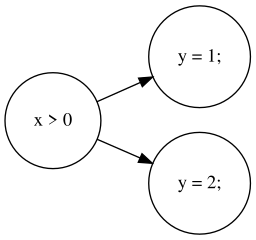
\includegraphics[width=0.5\textwidth]{Images/sample_edge_graph.png}
    \caption{Example of edge between basic blocks}
    \label{fig:sample_edge_graph}
\end{figure}
\phantom{}\\
When an edge is executed, the corresponding bit in the coverage map is incremented by \textit{+1} (to mark as ``\textit{hitted}"). The fuzzer uses this information to guide the generation of new test cases that maximize the coverage.
\\Within this action a coverage-guided fuzzer maintains a collection of inputs called \textbf{corpus}. In particular it is a collection of:
\begin{itemize}
    \item \textbf{Seeds}: Initial inputs that are used to start the fuzzing process.
    \item \textbf{Interesting inputs}: Inputs that are generated by the fuzzer during the fuzzing process and achieve new coverage (i.e. by mutating the seeds).
\end{itemize}
The corpus grows as the fuzzer adds new inputs that has allowed it to increase the coverage of the program.

\section{Stateful Fuzzing: Concepts and Challenges}
\textit{Stateless fuzzing} is a traditional fuzzing technique that generates random inputs to test the behavior of an application. However, this approach is not always effective for applications that maintain internal states across multiple interactions.
\\For example cosidering an FTP server, like \textbf{LightFTP} (\href{https://github.com/hfiref0x/LightFTP}{https://github.com/hfiref0x/LightFTP}), until the user is not authenticated, all the inputs are meaningless. In this case, the fuzzer should be able to generate a sequence of inputs that first authenticate the user and then test the behavior of the application.
\textit{Stateful fuzzing} adds state awareness to traditional fuzzing methods. It considers an application's internal state and how that state might affect subsequent inputs handling. This becomes particularly critical for applications that handle complex state information, such as network servers, databases and interactive applications.

\subsection{Understanding Stateful Applications}
Stateful applications maintain state across multiple interactions or sessions. Examples include network servers that manage connection states, authentication states, session identifiers, or other state information specific to an application. These states significantly influence the processing of inputs and the behavior of the application over time.
\\Good practices in state transition management are crucial for both security and reliability: bugs related to state transitions can lead to vulnerabilities such as unauthorized access, denial of service \textit{(DoS)}, or data corruption. 
\\Stateful fuzzers attempt to model and explore these state transitions by generating input sequences that mimic valid usage scenarios while concurrently monitoring state changes to ensure comprehensive coverage of all possible transitions. To better understand this concept, consider a simple state model shown in Figure \ref{fig:simplestatemodel}.
%TODO fix figure
\begin{figure}[h]
    \centering
    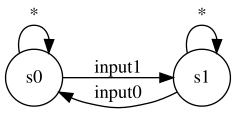
\includegraphics[width=0.5\textwidth]{Images/simplestatemodel.png}
    \caption{A simple state model illustrating state transitions in a stateful application}
    \label{fig:simplestatemodel}
\end{figure}


\subsection{Key Techniques in Stateful Fuzzing}
Stateful fuzzing involves several advanced techniques that distinguish it from traditional fuzzing approaches (\textit{The Art, Science, and Engineering of Fuzzing} \cite{theartoffuzzing}):

\begin{itemize}
    \item \textbf{State Modeling}: The process of building a model representing an application state machine by reverse engineering source code, observing real interactions, or guide test case generation in conjunction with machine learning techniques.
    
    \item \textbf{State Tracking}: This involves tracking the state of the application across successive inputs; indeed, tracking of network traffic, system calls, or internal state variables.
    
    \item \textbf{Feedback Mechanisms}: With feedback mechanisms, one can prioritize those test cases that tend to explore new states or code paths; hence, the general efficiency of fuzzing can be improved.
    
    \item \textbf{Sequence Generation}: It is the need to generate input sequences to properly model actual use, since the findings of vulnerabilities often depend on specific sequences or state transitions.
    
    \item \textbf{Learning-Based Approaches}: Certain fuzzers utilize machine learning or heuristic methodologies to dynamically ascertain the structural configuration of the application's state machine, thereby enabling the fuzzer to adjust and enhance its efficacy progressively.
\end{itemize}

\subsection{Challenges in Stateful Fuzzing}
Successfully performing testing is fraught with several challenges in stateful fuzzing (\textit{Is Stateful Fuzzing Really Challenging?} \cite{statefulfuzzingchallenges}):

\begin{itemize} 
    \item \textbf{State Explosion}: As in real life, an application itself may have a number of possible states and with more states, a risk for exponential growth in process complexity increases. In this case, state abstraction, pruning, or prioritization counters the \textit{state explosion} in an essential way.
    
    \item \textbf{Protocol Complexity}: Generating meaningful input sequences can involve deep knowledge of complex protocols or state machines. This often includes much domain-specific knowledge or even advanced algorithms.
    
    \item \textbf{Performance Overhead}: To date, state tracking performed by the application and input sequence generation can cause significant computational costs, hence slowing down the fuzzing process.

    \item \textbf{Handling Non-Deterministic Behavior}: The nondeterministic behavior of stateful applications often results from concurrency, differences in external inputs, or even timing variations. These factors therefore make the reproduction of bugs and receiving consistent fuzzing results usually difficult.

\end{itemize}

\section{Lighttpd: A Case Study for Stateful Fuzzing}
Lighttpd is an open-source web server optimized for performance with very low memory usage. It is designed to handle huge volumes of parallel connections with minimal overhead, making it particularly useful on systems with limited resources or those requiring a high degree of concurrency. Its modular design and support for advanced web protocols make it a popular choice for embedded systems, cloud computing platforms and high-traffic websites. It was used by popular websites like Wikimedia, YouTube and SourceForge, nowadays is used in general for ...%TODO add more

\subsection{Overview of Lighttpd Architecture}
Lighttpd operates on an event-driven architecture, which enables it to serve many requests concurrently. An asynchronous I/O framework is employed to minimize overhead in network connections, allowing the server to scale efficiently under varying workloads. The key features of Lighttpd include:

\begin{itemize}
    \item \textbf{Modular Design}: Provides a series of modules for implementing functions like \textit{URL rewriting}, \textit{HTTP compression}, \textit{SSL/TLS and WebSockets}. The modular design allows for customization based on specific needs.
    
    \item \textbf{Protocol Support}: Out of the box, it supports \textit{HTTP/1.1, HTTPS, FastCGI, SCGI and HTTP/2}, making it suitable for a wide range of web applications and services.
    
    \item \textbf{Security Attributes}: Advanced integrated security features include TLS/SSL encryption, prevention of \textit{denial-of-service} attacks and multiple authentication options.
\end{itemize}

\subsection{Relevance of Lighttpd for Fuzzing}

Lighttpd is an important SUT for fuzzing due to its common use behind various internet applications.
These characteristics make it a suitable candidate for evaluating fuzzing techniques.
By default, Lighttpd is maintains transient states during the processing of requests (Figure \ref{fig:lighttpdstatemodel}).
\begin{figure}[H]
    \centering
    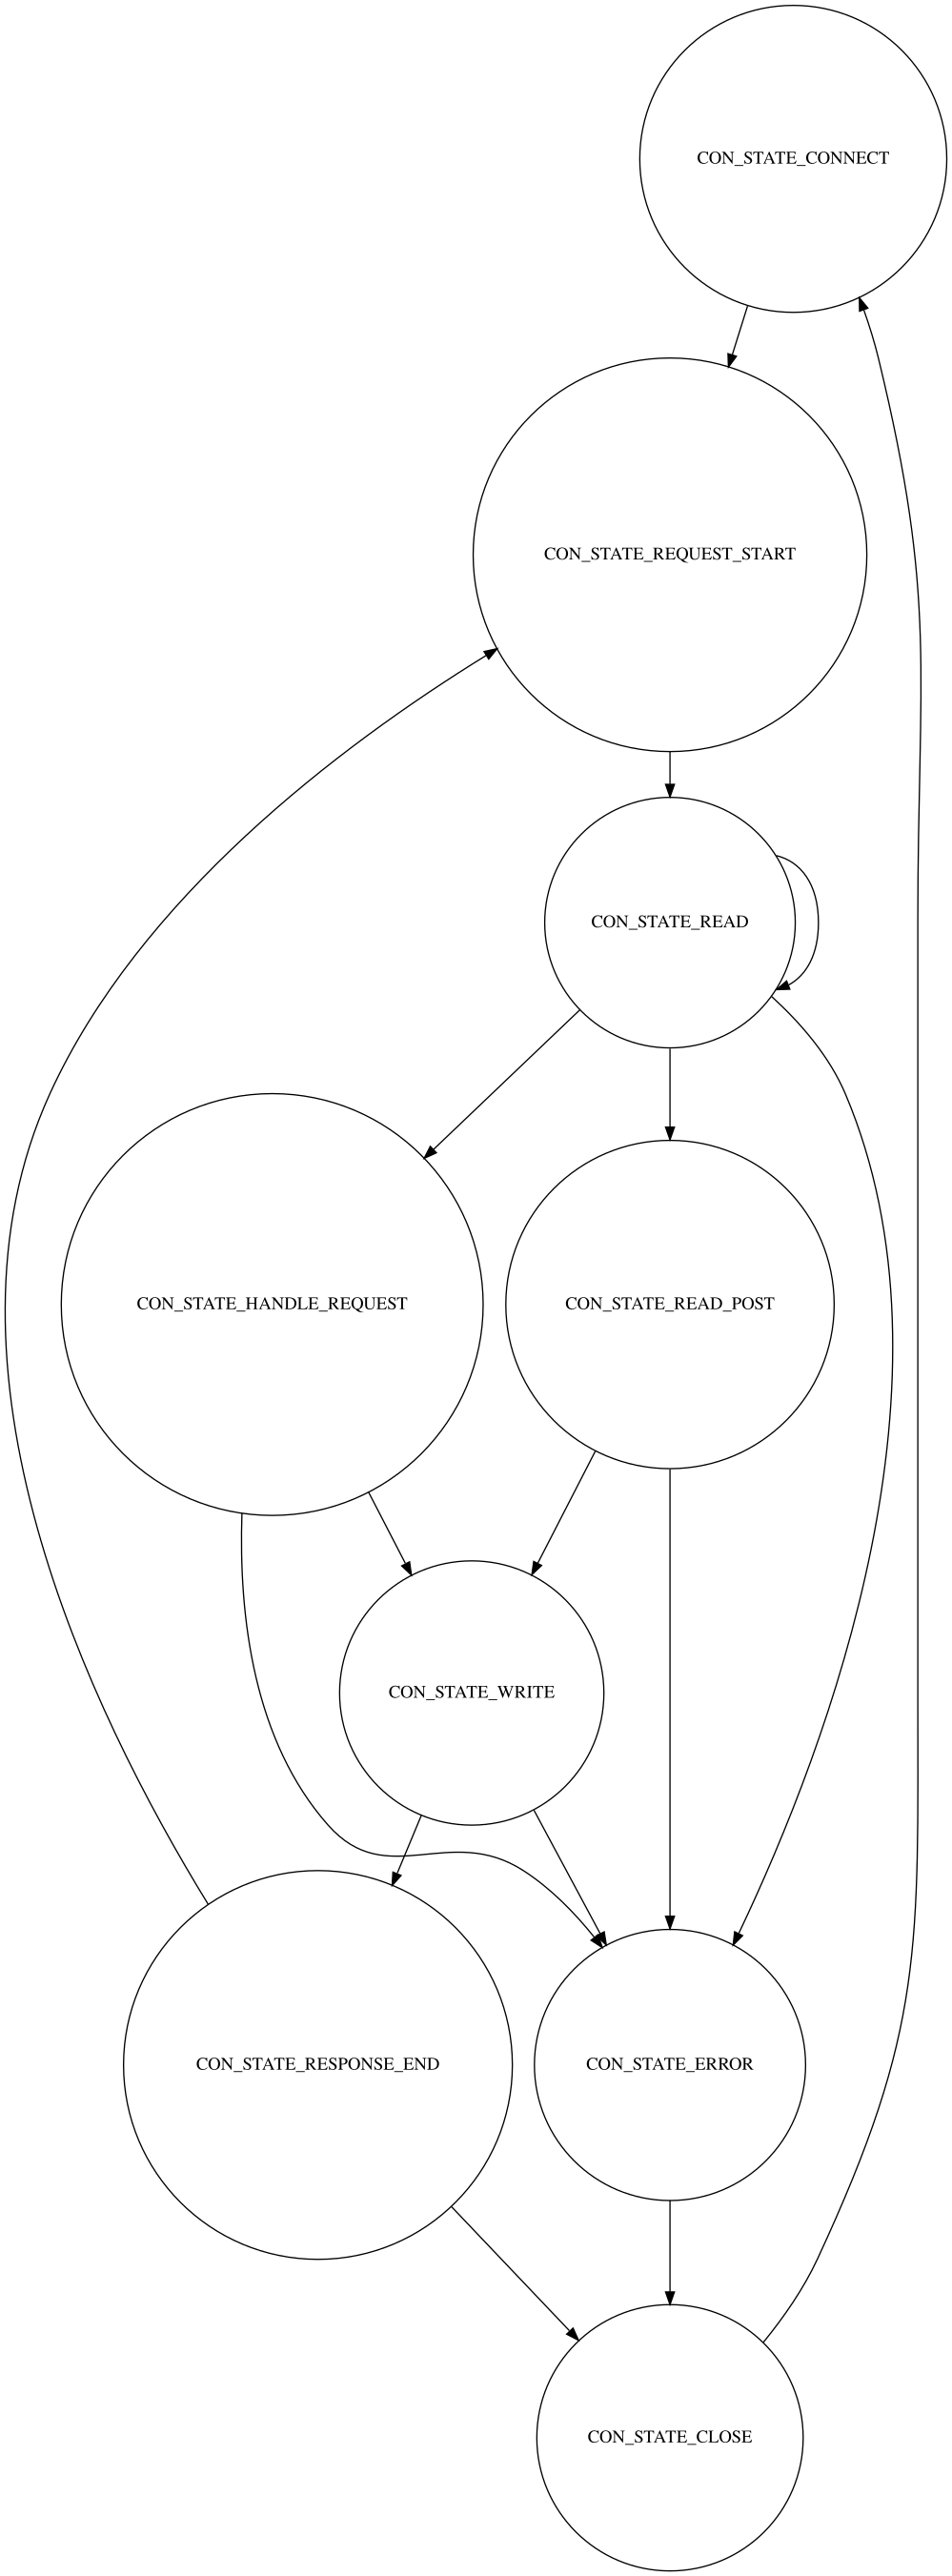
\includegraphics[width=0.6\textwidth]{Images/lighttpd_original.png}
    \caption{State model of Lighttpd}
    \label{fig:lighttpdstatemodel}
\end{figure}
\phantom{}\\
The state model seems to be complex, but the state are effectively transitory.
\\A sample flow of states in Lighttpd is as follows:
\begin{itemize}
    \item \textbf{1.CON\_STATE\_CONNECT}: The initial default state before a connection is established.
    
    \item \textbf{2.CON\_STATE\_REQUEST\_START}: The state right after a connection is established and wait for request.
    
    \item \textbf{3.CON\_STATE\_READ}: The state when the server is reading the request (here the server can be in a loop to read the request).
    
    \item \textbf{4.CON\_STATE\_HANDLE\_REQUEST}: The state when the server is processing the request, if body length is null.
    
    \item \textbf{4.CON\_STATE\_READ\_POST}: The state when the server is processing the request, if body length is more than 0.
    
    \item \textbf{5.CON\_STATE\_WRITE}: The state when the server is writing the response.
    \item \textbf{6.CON\_STATE\_ERROR}: The state when an unhandled error occurs.
    
    \item \textbf{7.CON\_STATE\_RESPONSE\_END}: The state after the request has been fully received.
    
    \item \textbf{8.CON\_STATE\_CLOSE}: The state when the connection is closed.
\end{itemize}
In the \textit{CON\_STATE\_CONNECT} ther is no control of input, because it only changes when the connection is established.
\\The only stationary state could be the \textit{CON\_STATE\_READ}, because it is a loop that reads the request (i.e. if the request is sent line by line, it will loop into it).
\\The other states are transitory because, at the end, it will go back to \textit{CON\_STATE\_REQUEST\_START} or \textit{CON\_STATE\_CONNECT}.
\\For this thesis, it has been chosen to model the state of the server based on the existence or non-existence of a resources (Figure \ref{fig:existent_nonexistent_resource_statemodel}). A resource can be a file, a directory, or any other entity that can be accessed via HTTP. By considering two types of requests—those that attempt to access an existing resource and those that attempt to access a non-existing resource—it can effectively explore different states of the server.

\section{Fuzzers Overview: AFLNet, ChatAFL and Fallaway}

For this thesis, three stateful fuzzers—AFLNet, ChatAFL and Fallaway—will be benchmarked over Lighttpd.
 
\subsection{AFLNet}
AFLNet \cite{AFLNet} is a stateful CGF tool. It integrates automated state model inference with coverage-guided fuzzing, creating a synergistic relationship between the two processes. As fuzzing generates new message sequences to reach unexplored states, it progressively builds a more complete state model. Concurrently, this dynamically evolving state model helps guide fuzzing efforts towards more significant areas of the code, leveraging both state and code coverage information of the retained message sequences.
\\AFLNet is implemented as an extension of the popular grey-box fuzzer AFL, with the additional capability of facilitating \textit{network communication} over sockets, which is not supported by the original AFL. To achieve this, AFLNet establishes two communication channels: one for sending messages to the SUT and another for receiving responses. The response-receiving channel acts as a state feedback channel, complementing the code coverage feedback channel utilized by other CGF tools. The communication is implemented using standard C Socket APIs and synchronization between AFLNet and the server is ensured by introducing delays between requests.
\\AFLNet uses a \textit{prefix-based fuzzing} strategy, where the fuzzer maintains a prefix of the message sequence that has been successfully processed by the server. This prefix is used to guide the generation of new message sequences, ensuring that the fuzzer explores new states and code paths while maintaining the validity of the input.
\\The seeds to AFLNet consists of \textit{pcap} files capturing network traffic, such as interactions between a client and server. A network sniffer, like \textit{tcpdump}, is used to capture realistic exchanges and a packet analyzer, such as Wireshark, can automatically extract the relevant message sequences. AFLNet uses a \textbf{Request Sequence Parser} to generate an initial corpus of message sequences by parsing these pcap files. It isolates individual client requests, discards the responses and identifies the beginning and end of each message, utilizing protocol-specific markers.
\\The \textbf{State Machine Learner} component then augments the protocol state machine with newly observed states and transitions by analyzing server responses. AFLNet extracts status codes from server responses to identify and document new states and transitions. The \textbf{Target State Selector} leverages this information to determine which state the fuzzer should focus on next. This is done by applying several heuristics based on the statistical data gathered from the state machine, aiming to identify ``blind spots" or rarely exercised states and maximize the discovery of new state transitions.
\\Once a target state is selected, the \textbf{Sequence Selector} chooses a corresponding message sequence from the corpus that can reach the desired state. AFLNet maintains a state corpus and a hashmap to facilitate efficient selection of sequences. The selected sequence is then subjected to mutation using the \textbf{Sequence Mutator}, which builds upon AFL's \textit{`fuzz\_one`} method (\textit{input selection, mutation, execution, feedback collecltion, minimization and prioritization, looping}). AFLNet uses \textit{protocol-aware} mutation operators to modify the candidate subsequence, enhancing the chances of generating new sequences that can lead to the discovery of new states or code branches.
\\AFLNet employs several mutation strategies, such as replacing, inserting, duplicating, or deleting messages, in addition to standard byte-level operations like bit flipping. Generated sequences deemed ``interesting" — those that uncover new states, transitions, or code branches — are added to the corpus for further fuzzing. This evolutionary approach, driven by the continuous enhancement of the message sequence corpus, underpins the effectiveness of AFLNet in achieving comprehensive state and code coverage.

\subsection{ChatAFL}
Traditional \textit{mutation-based protocol fuzzing} relies heavily on recorded message sequences to generate test cases, which can limit its effectiveness in thoroughly exploring the input and state space of complex network protocols. Existing approaches often require detailed, \textit{machine-readable} protocol specifications, which are labor-intensive to produce and maintain. Furthermore, these approaches may struggle with limited seed diversity and may reach a coverage plateau (no more progress in discovering code paths or states), where further exploration yields diminishing returns.
\\To address these limitations, recent advancements have explored the potential of \textit{Large Language Models (LLMs)} \cite{minaee2024largelanguagemodelssurvey} to assist in the fuzzing process.
\\LLMs are a class of neural network models that have demonstrated remarkable capabilities in natural language understanding and generation. They can be fine-tuned for specific tasks and have been successfully applied to a wide range of applications, including language translation, text generation and code completion.
\\LLMs are pre-trained on extensive corpora, including publicly available protocol specifications and have demonstrated impressive capabilities in understanding and generating text. This presents an opportunity to leverage LLMs to improve fuzzing strategies by interpreting natural language descriptions of protocols and generating structured, diverse message sequences.
\\\textit{LLM-guided protocol fuzzing} uses the capabilities of LLMs to overcome the limitations of traditional mutation-based fuzzers. This method is implemented in ChatAFL \cite{chatafl} , a fuzzing tool built upon the AFLNet framework. ChatAFL incorporates LLMs to assist in three key areas:

\begin{enumerate}
    \item \textbf{Grammar Extraction:} By querying the LLM, the fuzzer can obtain a machine-readable grammar for the protocol under test. This grammar is used to guide mutations in a way that maintains the structural validity of the messages, thus enhancing the fuzzer's ability to explore new state transitions.

    \item \textbf{Seed Enrichment:} The LLM is used to diversify the initial seed corpus by generating new message types that are contextually relevant to the protocol. This helps to overcome the limitations posed by a narrow set of initial test cases and increases the likelihood of discovering new protocol behaviors.

    \item \textbf{Breaking Coverage Plateaus:} When the fuzzer is unable to achieve further state or code coverage, it is considered to be in a coverage plateau. The LLM can be prompted to generate new message sequences aimed at escaping the plateau by triggering unexplored state transitions.
\end{enumerate}
The integration of LLMs into protocol fuzzing offers several benefits:
\begin{enumerate}
    \item It reduces the dependence on pre-existing machine-readable protocol specifications by leveraging natural language processing capabilities.
    \item It enhances the diversity and effectiveness of the fuzzing process by generating a wider variety of input sequences.
    \item It aligns with the inherent goals of fuzzing — automation and adaptability — by using LLMs that can be easily guided via prompts to perform specific tasks without extensive reprogramming or manual intervention.
\end{enumerate}
Overall, this LLM-guided approach, as demonstrated in ChatAFL, represents a novel direction in protocol fuzzing, combining traditional techniques with \textit{state-of-the-art} language models to improve both the breadth and depth of fuzzing campaigns.


\subsection{Fallaway}
Fallaway \cite{Fallaway} is a stateful fuzzer designed to address several key challenges faced by traditional fuzzers when handling stateful SUTs. Unlike stateless fuzzers such as AFL, which send single test cases and expect the SUT to terminate, Fallaway manages multiple states by incorporating a \textit{dual-loop} structure: an outer loop that selects the SUT state and an inner loop that sends multiple test cases for the chosen state. This approach helps maintain deliberate focus on specific states, prevents interference between states and ensures that progress in one state does not hinder progress in another.
\\To achieve these objectives, Fallaway decouples the concepts of state scheduling and test case (seed) scheduling.
The fuzzer has a \textbf{queue}, that is a scheduling algorithm that selects the next input to use based on different strategies like:
\begin{itemize}
    \item \textbf{Coverage-Yield (CY)} strategy, which uses a round-robin approach to select the next input to mutate.
    \item \textbf{Outgoing Edges (OE)} strategy, which prioritizes inputs that exercise new edges in the program (this is done by using metadata that keeps track of the outgoing edges of each state in the program and selecting the input that exercises the most new edges).
\end{itemize} 
Corpus and queue are used interchangeably, but they are not really the same thing. \\We can look at the queue as a mapping of the corpus within a scheduling algorithm to choose the next input to mutate.
\\These are some examples of coverage-guided strategies:
\begin{itemize}
    \item \textbf{Multiple Corpus Single Map (MCSM)}: This strategy uses a single coverage map to track the coverage of the program and multiple queues to store the inputs (is more efficient in terms of memory usage and faster in terms of execution time, but it is less effective in terms of coverage).
    
    \item \textbf{Multiple Corpus Multiple Map (MCMM)}: This strategy uses multiple coverage maps to track the coverage of the program and multiple queues to store the inputs (is more effective in terms of coverage, but it is less efficient in terms of memory usage and slower in terms of execution time).
\end{itemize}
Each queue contains inputs that have allowed the fuzzer to reach a specific state of the program. The fuzzer uses a scheduler to select which input to mutate next based on the coverage achieved by the input.
\\For each state, a unique prefix is maintained along with a separate corpus of test cases, allowing focused exploration of the SUT's behavior within that state. Observations and feedback are also stored separately for each state, avoiding the problem of feedback contamination across different states. This strategy enables the fuzzer to maintain a clear distinction between the information gathered in each state, ensuring that the testing process remains unbiased and effective.
\\Fallaway is built on the \textbf{LibAFL} \cite{libafl} framework, which is a modular library for developing fuzzers. To make LibAFL suitable for stateful SUTs, Fallaway extends its functionality in two key ways:
\begin{enumerate}
    \item It uses AFL's \textbf{persistent mode}, designed to keep a SUT application running continuously between different test cases, rather than starting a new process for each test case. This approach is particularly useful for maintaining and manipulating the application's state across test cases, allowing the SUT to handle inputs continuously without resetting after each test case, which is crucial for efficient fuzzing of stateful systems.
    \item It introduces an outer loop to handle state transitions and reset the SUT accordingly, ensuring compatibility with LibAFL's existing mechanisms for executing test cases.
\end{enumerate}  
By integrating these methods, Fallaway leverages the speed and efficiency of persistent mode fuzzing while maintaining precise control over state transitions. This approach allows it balance execution speed and focus state exploration.

\chapter{Setup and fuzzing}
\label{chap:Setup}

\section{Fallaway}
Fallaway use the \textbf{persistent mode}. This mode allows the fuzzer to maintain the server's state across multiple requests, which is especially useful in scenarios where the server does not reset its state between requests, such as when managing user sessions or maintaining authentication states in a web application.
\\The persistent mode is implemented by modifying the Lighttpd server to maintain its state between requests. The server operates in a separate process and the fuzzer interacts with it via a socket. The fuzzer sends requests to the server and receives responses, using the results to guide the generation of subsequent requests. This process continues in a loop until the fuzzing session is complete.
\\To enable this, it is necessary to modify the Lighttpd code to ensure that the server continuously receives, processes and responds to requests without shutting down. The changes are made to the function \textit{server\_main\_loop} in the \textit{src/server.c} file and to the connection handling functions in \textit{src/connections.c} of the Lighttpd source code. The specific code changes are shown in the next section, providing a comparison between the original and modified code.

\subsection{Lighttpd Code Modifications for Persistent Mode}

Table \ref{tab:connections_patch} presents a comparison of the original and modified code for the \textit{connections.c} file. The modifications to this file are crucial for maintaining an open connection state, ensuring that the fuzzer can interact continuously with the server. It is also important to clean all buffers and old data for that connection.
\\Table \ref{tab:server_patch} shows a comparison of the original and modified code for the \textit{server.c} file. The changes made here are essential for enabling persistent server operation, allowing the fuzzer to manage and maintain server state across multiple requests, looping into the \textit{\_\_AFL\_LOOP}.

\begin{table}[H]
\centering
\begin{tabular}{|p{0.9\textwidth}|}
\hline
\textbf{Original Code} \\
\hline
\begin{lstlisting}[language=c, basicstyle=\footnotesize, breaklines=true]
static void connection_handle_shutdown(connection *con) {
    ...
    connection_reset(con);
    
    /* close the connection */
    if (con->fd >= 0 
        && (con->is_ssl_sock 
        || 0 == shutdown(con->fd, SHUT_WR))) {
        con->close_timeout_ts = log_monotonic_secs;

        request_st * const r = &con->request;
        connection_set_state(r, CON_STATE_CLOSE);
        if (r->conf.log_state_handling) {
            log_error(r->conf.errh, __FILE__, __LINE__,
                "shutdown for fd %d", con->fd);
        }
    } else {
        connection_close(con);
    }
}
\end{lstlisting} \\
\hline
\textbf{Modified Code} \\
\hline
\begin{lstlisting}[language=c, basicstyle=\footnotesize, breaklines=true]
static void connection_handle_shutdown(connection *con) {
    ...
    connection_reset(con);

    /* keep the connection open and reset it */
    request_reset_ex(&con->request);
    chunkqueue_reset(con->read_queue);
    con->request_count = 0;
    con->is_ssl_sock = 0;
    con->revents_err = 0;
    connection_set_state(&con->request,CON_STATE_REQUEST_START);
}
\end{lstlisting} \\
\hline
\end{tabular}
\caption{Comparison of Original and Modified Code for `src/connections.c`}
\label{tab:connections_patch}
\end{table}

\begin{table}[H]
\centering
\begin{tabular}{|p{0.9\textwidth}|}
\hline
\textbf{Original Code} \\
\hline
\begin{lstlisting}[language=c, basicstyle=\footnotesize, breaklines=true]
static void server_main_loop (server * const srv) {
    ...
    server_load_check(srv);

    #ifndef _MSC_VER
    static
    #endif
    connection * const joblist = log_con_jqueue;
    log_con_jqueue = sentinel;
    server_run_con_queue(joblist, sentinel);

    if (fdevent_poll(srv->ev, log_con_jqueue != sentinel ? 0 : 1000) > 0)
        last_active_ts = log_monotonic_secs;
}
\end{lstlisting} \\
\hline
\textbf{Modified Code} \\
\hline
\begin{lstlisting}[language=c, basicstyle=\footnotesize, breaklines=true]
static void server_main_loop (server * const srv) {
    ...
    server_load_check(srv);

    while (__AFL_LOOP(INT64_MAX)) {
        fdevent_poll(srv->ev, -1);
        
        #ifndef _MSC_VER
        static
        #endif
        connection * const joblist = log_con_jqueue;
        log_con_jqueue = sentinel;
        server_run_con_queue(joblist, sentinel);
    }

    srv_shutdown = 1;
}
\end{lstlisting} \\
\hline
\end{tabular}
\caption{Comparison of Original and Modified Code for `src/server.c`}
\label{tab:server_patch}
\end{table}

\subsection{Setting Up the Fuzzing Environment}

To run the fuzzer, it is important to build a Docker container that includes all the necessary dependencies and the modified Lighttpd server. The Dockerfile below is based on an image that already contains Fallaway and shows the steps to set up this environment.

\begin{lstlisting}
FROM fallaway 

WORKDIR /

# Copy the patch file
COPY ./lighttpd.patch /lighttpd.patch

ENV DEBIAN_FRONTEND=noninteractive

# Install lighttpd dependencies
RUN apt-get install -y \
    autoconf \
    automake \
    libtool \
    m4 \
    pkg-config \
    libpcre2-dev \
    zlib1g-dev \
    zlib1g \
    openssl \
    libssl-dev \
    scons

# Create the root directory for the server
RUN chmod 777 /tmp

# Install

# Set up environment variables for ASAN
ENV ASAN_OPTIONS='abort_on_error=1:symbolize=0:detect_leaks=0:detect_stack_use_after_return=1:detect_container_overflow=0:poison_array_cookie=0:malloc_fill_byte=0:max_malloc_fill_size=16777216'

# Download lighttpd
ENV CC=afl-cc
ENV CXX=afl-cc
RUN git clone https://git.lighttpd.net/lighttpd/lighttpd1.4.git lighttpd
WORKDIR /lighttpd 
RUN git checkout 9f38b63cae3e2
RUN git apply /lighttpd.patch
RUN ./autogen.sh  
RUN scons CC=/AFLplusplus/afl-cc CXX=/AFLplusplus/afl-cc -j 4 build_static=1 build_dynamic=0
RUN mv /lighttpd/sconsbuild/static/build/lighttpd /lighttpd/lighttpd

# Copy the corpus
COPY ./corpus /corpus

# Copy the config file
COPY ./lighttpd.conf /lighttpd.conf

# Copy the run script
COPY ./run.sh /Fallaway/run.sh
# Make it executable
RUN chmod +x /Fallaway/run.sh

WORKDIR /Fallaway
\end{lstlisting}
\phantom{}\\
The Docker container is configured with all the dependencies to run the fuzzer and build the modified Lighttpd server, providing a controlled environment to conduct the fuzzing experiment.
Another important file to consider is the configuration file of the Lighttpd server, which is shown below.\\
\begin{figure}[H]
\begin{lstlisting}
    server.document-root = "/tmp"
    server.bind = "0.0.0.0"
    server.port = 8080
    mimetype.assign = (".txt" => "text/plain", ".html" => "text/html" )

    server.max-worker = 1 
    server.max-connections = 1000
\end{lstlisting}
\caption{Lighttpd configuration file}
\label{fig:lighttpd_conf_fallaway}
\end{figure}
\phantom{}\\
This configuration file specifies the server's document root, bind address, port, and maximum number of workers and connections. By defining these parameters the server will operates correctly and can handle the incoming requests from the fuzzer.
\\In particular, it is forced to have just one worker to avoid problems with fuzzing, because Fallaway is not designed to work with multi-process SUT.

\subsection{Mutator and Corpus}

Another crucial aspect of the fuzzing process involves the corpus and the mutator. In this experiment, it has been defined the state of the server based on the existence \ref{tab:existent_resource} or non-existence \ref{tab:nonexistent_resource} of a resource. Specifically considering two types of requests: one that attempts to access a resource that exists and another that attempts to access a resource that does not exist.
\\\\The \textbf{corpus} folder consists of: a set of folders, one for each state, each containing a set of files, the \textit{prefixes}, that are a sequence of messages to reach that state.
\\In this case, the corpus is composed by two folders: one for the existent resource and one for the non-existent resource. Each folder contains a single file with a request to reach the state.
Here we have two requests for the two states:
\begin{figure}[H]
    \centering
    \begin{adjustbox}{valign=t}
    \begin{lstlisting}
    PUT /hello.txt HTTP/1.1
    Host: 127.0.0.1:8080
    Content-type: text/plain
    Content-length: 13

    Hello, World!

    
    \end{lstlisting}
    \end{adjustbox}
    \caption{Existent resource request}
    \label{tab:existent_resource}
\end{figure}
    
\begin{figure}[H]
    \centering
    \begin{adjustbox}{valign=t}
    \begin{lstlisting}
    DELETE /hello.txt HTTP/1.1
    Host: 127.0.0.1:8080
    User-Agent: curl/8.0.1
    Accept: */*

    
    \end{lstlisting}
    \end{adjustbox}
    \caption{Non-existent resource request}
    \label{tab:nonexistent_resource}
\end{figure}
\phantom{}\\
The \textbf{mutator}, responsible for generating variations of the requests, is relatively straightforward. Its primary function is to modify the existing requests by appending the sequence of characters ``\textit{\textbackslash r\textbackslash n\textbackslash r\textbackslash n}" to the end of each request. This modification is essential as it ensures that the requests are well-formed and adhere to HTTP protocol standards.
\\Before this, the mutator adds a set of tokens (taken from files in the corpus folder, but outside of the state folder) and places them in random positions within the request.
\\By ensuring the requests are properly formatted, the mutator enables the server to parse and process them correctly, which is vital for accurate fuzz testing.
\\An example of the corpus folder is as follows:
\begin{figure}[H]
    \centering
    \begin{adjustbox}{valign=t}
    \begin{lstlisting}
    corpus
    |-- existent_resource
    |   |-- 0_put
    |   |-- metadata
    |-- non_existent_resource
    |   |-- 0_delete
    |   |-- metadata
    |-- GET
    |-- DELETE
    |-- PUT
    |-- OPTIONS
    |-- POST
    \end{lstlisting}
    \end{adjustbox}
    \caption{Corpus folder structure}
\end{figure}
\phantom{}\\
Summing up: \textit{existent\_resource} folder is a state, \textit{0\_put} is a prefix to reach that state and, in this case is the full request to reach it. The same for \textit{non\_existent\_resource} and \textit{0\_delete}. The \textit{metadata} files contains the number of outgoing edges for that state. In this case, the number of outgoing edges is 2 for both states, because we can have:
\begin{itemize}
    \item \textit{existent\_resource} state: when sending the put request, the server can return a 404 error, if the resource exists, or can return a 200 OK.
    \item \textit{non\_existent\_resource} state: when sending the delete request, the server can return a 404 error, if the resource does not exist, or can return a 200 OK.
\end{itemize}
\phantom{}\\
Finally the other files rapresent the tokens that the mutator will use to generate new requests.

\subsection{Fuzzing Execution}

To run the fuzzer for 24 hours, it is necessary to run the following script:
\begin{figure}[H]
    \begin{lstlisting}
    #!/bin/bash
    bin="${1:-mcsm-cy}"
    loops="${2:-1000}"

    timeout 24h cargo run --release --bin fallaway-http-$bin -- --in-dir /corpus --out-dir /output_lighttpd --target-port 8080 --loops $loops -t 300 /lighttpd/lighttpd -D -f /lighttpd.conf
    \end{lstlisting}
    \caption{Execution script}
    \label{fig:exec_script_fallaway}
\end{figure}
In particular there are:
\begin{itemize}
    \item \textbf{timeout 24h}: a timeout of 24h for the next command.
    \item \textbf{cargo run}: the command to run the fuzzer.
    \item \textbf{--release}: the flag to run the fuzzer in release mode.
    \item \textbf{--bin fallaway-http-\$bin}: the state scheduler strategy (by default is mcsm-cy).
    \item \textbf{--}: the flag to separate the fuzzer arguments from the binary arguments.
    \item \textbf{--in-dir /corpus}: the input directory for the fuzzer.
    \item \textbf{--out-dir /output\_lighttpd}: the output directory for the fuzzer, where the results will be stored.
    \item \textbf{--target-port 8080}: the port of the server.
    \item \textbf{--loops \$loops}: the number execution the fuzzer will do before changing state (the \textit{\_\_AFL\_LOOP} is bigger volountarly, so that we prioritize this argument).
    \item \textbf{-t 300}: the timeout for each test case, in milliseconds, which will trigger if the fuzzer does not reach the end of the \textit{\_\_AFL\_LOOP} in time.
    \item \textbf{/lighttpd/lighttpd -D -f /lighttpd.conf}: the command to run the server, in detached mode, with the configuration file.
\end{itemize}
The results of the fuzzing process will be discussed in the Chapter \ref{chap:Results}.

\section{AFLNet and ChatAFL}

\subsection{Setting Up the Fuzzing Environment}

Both AFLNet and ChatAFL are built and configured using \textbf{ProFuzzBench} ~\cite{profuzzbench}, a benchmark suite specifically designed for evaluating network protocol fuzzers. ProFuzzBench provides a standardized environment and set of targets to ensure a fair comparison among different fuzzers.
\\By using ProFuzzBench, AFLNet and ChatAFL benefit from a streamlined setup process that automates the installation of dependencies and configuration of the environment, thus reducing setup overhead. This setup also involves additional dependencies, such as specific Python packages, which are necessary for supporting ChatAFL's unique capabilities like leveraging language models internally.
\\The Docker setup derived from ProFuzzBench provides the same base environment for both AFLNet and ChatAFL, ensuring compatibility and consistency across experiments. By using this common benchmark suite, researchers can directly compare results, further validating the effectiveness and performance differences between the fuzzers.
Another important thing to consider is the configuration file of the Lighttpd server, which is shown below.\\
\begin{figure}[H]
    \begin{lstlisting}
        server.document-root = "/tmp"
        server.bind = "127.0.0.1"
        server.port = 8080
        mimetype.assign = (".txt" => "text/plain", ".html" => "text/html" )
    \end{lstlisting}
    \caption{Lighttpd configuration file}
    \label{fig:lighttpd_conf_aflnetchatafl}
\end{figure}

\subsection{Mutator and Corpus}

AFLNet and ChatAFL use a corpus of test cases to seed the fuzzing process. However, their approach to handling and mutating this corpus differs slightly:

\begin{itemize}
    \item \textbf{AFLNet}: Focuses on network protocol fuzzing by analyzing and mutating protocol-specific fields in input messages. The corpus for AFLNet includes various protocol messages (e.g., HTTP requests) that are tailored to network targets. AFLNet leverages coverage feedback as well as response error codes from the server to refine its mutations and generate new test cases.

    \item \textbf{ChatAFL}: Enhances the mutation process using a language model (LLM) to generate intelligent mutations. This approach allows it to craft inputs that are more likely to uncover new code paths or trigger complex behaviors. The LLM is used to predict and prioritize inputs based on semantic understanding of the protocol or application under test.
\end{itemize}

Here are some examples of the corpus used by AFLNet and ChatAFL:
\begin{figure}[H]
    \centering
    \begin{adjustbox}{valign=t}
    \begin{lstlisting}
    GET /hello.txt HTTP/1.1
    Host: 127.0.0.1:8080
    User-Agent: curl/8.0.1
    Accept: */*
        
            
    \end{lstlisting}
    \end{adjustbox}
    \caption{Seed used by AFLNet and ChatAFL}
\end{figure}

\begin{figure}[H]
    \centering
    \begin{adjustbox}{valign=t}
    \begin{lstlisting}
    OPTIONS /hello.txt HTTP/1.1
    Host: 127.0.0.1:8080
    User-Agent: curl/8.0.1
    Accept: */*

    
    \end{lstlisting}
    \end{adjustbox}
    \caption{Seed used by AFLNet and ChatAFL}
\end{figure}

\begin{figure}[H]
    \centering
    \begin{adjustbox}{valign=t}
    \begin{lstlisting}
    DELETE /hello.txt HTTP/1.1
    Host: 127.0.0.1:8080
    User-Agent: curl/8.0.1
    Accept: */*

    
    \end{lstlisting}
    \end{adjustbox}
    \caption{Seed used by AFLNet and ChatAFL}
\end{figure}
\phantom{}\\
AFLNet and ChatAFL also use a dictionary during fuzzing, shown in Figure \ref{fig:dictionary}. This dictionary is used to generate meaningful and diverse input cases, ensuring that the fuzzer explores a wide range of scenarios and protocols. By leveraging such a dictionary, these tools enhance their ability to cover different code paths.
\begin{figure}[H]
    \centering
    \begin{adjustbox}{valign=t}
    \begin{lstlisting}
    "GET"
    "PUT"
    "POST"
    "OPTIONS"
    "127.0.0.1"
    "DELETE"
    "CONNECT"
    "TRACE"
    "HEAD"
    "hello.txt"
    "User-Agent"
    "StarWars3.wav"
    \end{lstlisting}
    \end{adjustbox}
    \caption{Dictionary used by AFLNet and ChatAFL}
    \label{fig:dictionary}
\end{figure}

\subsection{Fuzzing Execution}

\begin{figure}[H]
    \begin{lstlisting}
        #!/bin/bash

        PFBENCH="$PWD/benchmark"
        cd $PFBENCH

        PATH=$PATH:$PFBENCH/scripts/execution:$PFBENCH/scripts/analysis
        NUM_CONTAINERS=$1
        TIMEOUT=$(( ${2:-1440} * 60))
        SKIPCOUNT="${SKIPCOUNT:-1}"
        TEST_TIMEOUT="${TEST_TIMEOUT:-5000}"

        export TARGET_LIST=$3
        export FUZZER_LIST=$4

        if [[ "x$NUM_CONTAINERS" == "x" ]] || [[ "x$TIMEOUT" == "x" ]] || [[ "x$TARGET_LIST" == "x" ]] || [[ "x$FUZZER_LIST" == "x" ]]
        then
            echo "Usage: $0 NUM_CONTAINERS TIMEOUT TARGET FUZZER"
            exit 1
        fi

        PFBENCH=$PFBENCH PATH=$PATH NUM_CONTAINERS=$NUM_CONTAINERS TIMEOUT=$TIMEOUT SKIPCOUNT=$SKIPCOUNT TEST_TIMEOUT=$TEST_TIMEOUT scripts/execution/profuzzbench_exec_all.sh ${TARGET_LIST} ${FUZZER_LIST}
    \end{lstlisting}
    \caption{Execution script}
    \label{fig:exec_script_aflnetchatafl}
\end{figure}

\phantom{}\\
This is the script defined by ChatAFL repository ~\cite{chataflgithub}, that internally uses ProFuzzBench's scripts to run the fuzzers ~\cite{chataflgithubprofuz}.
\\An example of execution line is like this:\\
\begin{lstlisting}
./run.sh  <container_number> <fuzzed_time> <subjects> <fuzzers>
\end{lstlisting}
\phantom{}\\
The script takes four arguments:\\
\begin{itemize}
    \item \textit{CONTAINER\_NUMBER}: the number of containers to use for the execution of the fuzzer.
    \item \textit{FUZZED\_TIME}: the time in minutes after which the execution of the fuzzer will be stopped.
    \item \textit{SUBJECTS}: a list of targets to fuzz.
    \item \textit{FUZZERS}: a list of fuzzers to use.
\end{itemize}
\phantom{}\\
The command to fuzz Lighttpd for 24h using both AFLNet and ChatAFL is:
\begin{lstlisting}
./run.sh 1 1440 lighttpd aflnet,chatafl
\end{lstlisting}
Results from both AFLNet and ChatAFL will be discussed in detail in Chapter \ref{chap:Results}.

\section{Comparisons}

AFLNet and ChatAFL provide alternative approaches to fuzzing that share certain characteristics with Fallaway, but also have distinct differences in their setup, configuration, and operational strategies. The purpose of this section is to outline the similarities and unique features of the fuzzers, including how they handle server responses and their internal mechanisms for optimizing fuzzing performance.

\subsection{Setup}
The setup process for AFLNet and ChatAFL is quite similar to that of Fallaway, given that all three fuzzers share a common Docker-based environment with the necessary dependencies.
\\However, AFLNet and ChatAFL are built on top of ProFuzzBench, which provides a standardized environment for network protocol fuzzing.

\subsection{Operational Differences: Code Handling and Analysis}
As seen in Figure \ref{fig:lighttpd_conf_fallaway} and Figure \ref{fig:lighttpd_conf_aflnetchatafl}, AFLNet and ChatAFL do not need to force the number of workers to 1, because they do not share the same problem as Fallaway, due to their managment of the SUT.
\\In particular, below are some key differences in how AFLNet, ChatAFL, and Fallaway guide the fuzzing process:

\begin{itemize}
    \item \textbf{AFLNet} and \textbf{ChatAFL}: Both tools incorporate error code analysis in their feedback loop. They monitor the response codes (such as HTTP 404, 500, etc.) returned by the server to understand which inputs trigger errors or unexpected states. This allows them to focus on generating inputs that might exploit these observed errors, thereby uncovering potential vulnerabilities.
    \item \textbf{Fallaway}: In contrast, Fallaway exclusively relies on coverage metrics to guide the fuzzing process. It focuses on maximizing the code paths exercised by the generated inputs without directly considering the response codes from the server. This approach enables it to explore new paths more thoroughly, but may overlook specific error states that are of interest for security testing.
\end{itemize}
Indeed, Fallaway distinguishes itself from other fuzzers like AFLNet or ChatAFL by using the \textit{persistent mode}.

\subsection{Execution}
Another difference is in the execution's scripts, shown in Figure \ref{fig:exec_script_fallaway} and Figure \ref{fig:exec_script_aflnetchatafl}.
While Fallaway uses a custom script to run the fuzzer, AFLNet and ChatAFL rely on ProFuzzBench's execution scripts to manage the fuzzing process. This difference reflects the unique design and integration of each fuzzer within the ProFuzzBench framework.

\chapter{Comparison with AFLNet and ChatAFL}

Setup of ChatAFL and AFLNet is similar to the one of Profuzzbench \cite{profuzzbench}, that is a benchmarking tool designed for stateful fuzzing of network protocols. It provides a suite of open-source network servers implementing popular protocols and includes tools to automate fuzzing experiments. Unlike other benchmarks focused on stateless programs, ProFuzzBench specifically addresses stateful protocol fuzzing, which requires considering the protocol states and combinations of multiple messages. The benchmark aims to support research in fuzzing techniques for protocol security testing and is open-source, inviting contributions for extending its range of targets.
\\The real difference from Fallaway is in the execution script that we can see here:
\begin{lstlisting}
    #!/bin/bash

    PFBENCH="$PWD/benchmark"
    cd $PFBENCH

    PATH=$PATH:$PFBENCH/scripts/execution:$PFBENCH/scripts/analysis
    NUM_CONTAINERS=$1
    TIMEOUT=$(( ${2:-1440} * 60))
    SKIPCOUNT="${SKIPCOUNT:-1}"
    TEST_TIMEOUT="${TEST_TIMEOUT:-5000}"

    export TARGET_LIST=$3
    export FUZZER_LIST=$4

    if [[ "x$NUM_CONTAINERS" == "x" ]] || [[ "x$TIMEOUT" == "x" ]] || [[ "x$TARGET_LIST" == "x" ]] || [[ "x$FUZZER_LIST" == "x" ]]
    then
        echo "Usage: $0 NUM_CONTAINERS TIMEOUT TARGET FUZZER"
        exit 1
    fi

    PFBENCH=$PFBENCH PATH=$PATH NUM_CONTAINERS=$NUM_CONTAINERS TIMEOUT=$TIMEOUT SKIPCOUNT=$SKIPCOUNT TEST_TIMEOUT=$TEST_TIMEOUT scripts/execution/profuzzbench_exec_all.sh ${TARGET_LIST} ${FUZZER_LIST}
\end{lstlisting}
An example of execution line is like this:
\begin{lstlisting}
./run.sh  <container_number> <fuzzed_time> <subjects> <fuzzers>
\end{lstlisting}
We can see that the script takes four arguments:
\begin{itemize}
    \item \textit{CONTAINER\_NUMBER}: the number of containers to use for the execution of the fuzzer
    \item \textit{FUZZED\_TIME}: the time in minutes after which the execution of the fuzzer will be stopped
    \item \textit{SUBJECTS}: a list of targets to fuzz
    \item \textit{FUZZERS}: a list of fuzzers to use
\end{itemize}
We ran the script with the following command (1440 is 24h in minutes):
\begin{lstlisting}
./run.sh 1 1440 lighttpd aflnet,chatafl
\end{lstlisting}
The results of the fuzzing process will be discussed in the next chapter.
\chapter{Conclusion} 
This thesis explored the effectiveness of three stateful fuzzing tools—Fallaway, AFLNet, and ChatAFL—when applied to the Lighttpd web server. The study aimed to evaluate each tool's focusing on aspects like coverage, efficiency, and adaptability.
\\\\We discussed the importance of stateful fuzzing, particularly for applications where internal states and state transitions significantly impact behavior, such as web servers and network-based applications. Stateful fuzzing techniques were shown to be crucial in effectively testing these SUTs, as they consider the influence of previous interactions on the application's current state.
\\\\The research also involved comparing the setup processes for each fuzzer. Each tool required a different configuration and environment setup to achieve optimal performance. For instance, Fallaway's modifications to Lighttpd required a persistent mode for maintaining server states across multiple requests, while AFLNet and ChatAFL leveraged network protocol benchmarks to facilitate efficient fuzzing.
\\\\Additionally, various graphs were presented to illustrate the comparative results of the fuzzers. These showed differences in execution counts, code coverage achieved over time, and other performance metrics, providing a clearer understanding of how each tool behaves in different scenarios.
\\\\Through experimentation, it was found that each fuzzer employs a distinct approach to address the challenges of testing applications with complex internal states. 
\\\\\textbf{Fallaway} was observed to extensively explore possible program behaviors, achieving broad coverage by conducting numerous test executions. Its method is advantageous in scenarios where a comprehensive examination of all potential states is crucial, despite its higher demand on computational resources.
\\\\On the other hand, \textbf{AFLNet} leveraged its specialization in network protocols to achieve meaningful results with fewer test cases. It effectively targeted specific parts of the code, making it suitable for applications that require testing of network-related functionalities. However, its narrower focus might limit its applicability to broader testing needs.
\\\\\textbf{ChatAFL} introduced an innovative strategy by incorporating advanced techniques to optimize input generation. This tool struck a balance between maximizing coverage and minimizing execution overhead, offering a versatile solution adaptable to various types of software.
\\\\The findings underscore the need to select the appropriate fuzzing tool based on specific requirements, such as the nature of the software, the testing objectives and available resources. The evaluation provided valuable insights into the relative strengths and limitations of each fuzzer, guiding the selection of the most effective approach for different scenarios.

\newpage
\bibliographystyle{unsrt}
\renewcommand{\bibname}{References}
\addcontentsline{toc}{chapter}{References}
\bibliography{bibliography}

\chapter*{Greetings}
\addcontentsline{toc}{chapter}{Greetings}

Vorrei ringraziare prima di tutto me stesso, per la dedizione e la costanza che ho messo in questo lavoro e in tutto il mio percorso universitario.
\\Per la perseveranza che ho avuto nei momenti di difficoltà, per la passione che ho in questo campo, per il non aver mai mollato e per il non aver mai smesso di credere in me stesso.
\\Ringrazio i miei genitori, per il sostegno che mi hanno dato in tutti questi anni, per avermi sempre supportato e per avermi sempre spronato a dare il meglio di me.
\\In particolare, grazie a mio padre, per avermi trasmesso la passione per l'informatica, per avermi guidato nella vita e per avermi sempre dato consigli preziosi. Se oggi sono qui, è grazie a te.
\\Ringrazio mia madre, che nonostante qualche battibecco, nonostante il suo essere "curtigghiara", mi ha sempre amato, mi ha sempre reso felice e mi protegge da tutto e tutti. La mamma è sempre la mamma, e tu sei la MIA.
\\Ringrazio mia sorella per avermi sempre ascoltato, per essere sempre al mio fianco, per il sostegno che mi ha sempre dato e per la gioia che ha trasmesso nel vedere i miei successi, per l'orgoglio che ha nei mie confronti, per la stima, l'affetto (non dimostrato a volte per la sua afefobia), la comprensione, i litigi.
Complici e complicati, ma sempre uniti. Ti voglio un mondo di bene.
\\Ringrazio la mia ragazza, per tutto l'amore che mi ha dato, per la pazieza che ha avuto nei momenti di stress, per i pianti fatti insieme e per tutti i nostri momenti felici. Sei unica e speciale, ti amo.
\\Ringrazio i miei animali, Miele, Nica, Tigro e Coco, per avermi sempre fatto compagnia, per avermi sempre fatto sentire amato e per avermi sempre fatto sorridere. Sono parte di me.
\\Ringrazio i miei amici, per essermi stati vicini e per aver creduto in me.
\\In particolare ringrazio Emanuele Catania, per la fratellanza che ci lega, per il supporto che ci siamo sempre dati nonostante la distanza. Sei e sarai sempre mio fratello, ti voglio bene e ricordati che "il tiro di Nino Bixio, secondo me", lo posso fare solo io.
\\Ringrazio Beatrice Boninelli, che nonostante la distanza, nonostante il sentirci poco e nonostante le nostre vite separate, mi ha sempre dimostrato affetto e stima. Sin dal primo superiore abbiamo creato un legame che non si è mai spezzato, ti voglio bene, conta sempre su di me.
\\Ringrazio Marcello Maugeri, il mio "advisor", per essere stato sempre un punto di riferimento in questi anni in università e non solo. Grazie per avermi sempre dato consigli ottimi per tutto quello che riguarda la mia carriera universitaria e lavorativa, grazie per il supporto durante la stesura della tesi, grazie per avermi motivato e farmi credere in me stesso. Sei e continuerai ad essere un esempio per me.
\\Ringrazio il mio relatore, il Prof. Giampaolo Bella, per avermi insegnato che bisogna combattere per ciò in cui si crede e che per fare questo lavoro, bisogna crederci e metterci tutto.
\\Infine, come non ringraziare il mio compagno di corso, di esami, di risate, di soddisfazioni e di sconfitte. Grazie a te Simone Furneri, per tutti questi anni di studio insieme, per ogni materia fatta insieme, per ogni presa in giro e per ogni momento passato insieme. Abbiamo dato sempre il massimo e siamo arrivati fin qui, insieme. Spero che tutto questo possa continuare anche in futuro, ti voglio bene, sei speciale.
\\Grazie a tutti, per avermi reso la persona che sono oggi.
\end{document}